\chapter[Gerenciamento do Projeto] {Gerenciamento do Projeto}

O gerenciamento deste projeto é realizado tendo como modelo de referência o PMBOK, que é um guia com um conjunto de práticas de gestão de projetos organizados pelo instituto PMI \cite{pmbok2004}.

Dentre os 9 planos previstos no PMBOK, para o processo em questão foram adotados os de Comunicação, Riscos e Custo, devido ao entendimento da equipe de que estes agregam maior valor a gerência do projeto, e que serão detalhados nos capítulos seguintes.

Além dos planos do PMBOK, o trabalho também foi estruturado de acordo com as responsabilidades das subáreas, foi desenvolvido uma EAP (Estrutura Analítica do Projeto) para gestão do escopo, e foi elaborado um cronograma do mesmo, que são detalhados nos sub-tópicos a seguir.

\section{Responsabilidades}
Visando o melhor gerenciamento do projeto, a equipe do projeto foi dividida em 4 subáreas. As subáreas definidas foram:
\begin{table}[h]
\caption{Subáreas do projeto}
\centering
\begin{tabular}{|c|c|c|} \hline
\textbf{Subárea} & \textbf{Função} & \textbf{Membros}\\ \hline                               
Eletrônica & Desenvolver o Sistema de controle e comunicação juntamente com os integrantes da engenharia de software & Everton Klysnney M. Nunes Gustavo Oliveira do Amaral\\ \hline
Energia & Alimentar o Sistema, realizar o dimensionamento dos motores, desenvolver um sistema de proteção e fabricar um carregador & Fabio Bassi Bornazzi Jair Jorge Medeiros Larissa Antonia Pereira Thaís Soares Monteiro\\ \hline
Estruturas & Construir a estrutura do robô, bem como a estrutura da estante & Filippe Henriques Leal Marcelo Assis da Silveira Victor da Cunha F. R. de Almeida\\ \hline
Software & Definir e implantar o sistema de interface com o usuário e os sistemas embarcados & Iago Rodrigues Gonçalves Karine Santos Valença Murilo Duarte Gonçalves
Pedro de Lyra\\ \hline
\end{tabular}
\end{table}

No projeto foram definidos líderes com o intuito de se ter membros responsáveis por acompanhar, cobrar os prazos do projeto, comunicar aos professores eventualidades, modificações no produto e dúvidas que surgirem durante os processos, além de facilitar o andamento do projeto, intermediando as comunicações entre as subáreas. A tabela x apresenta os líderes do projeto:

\begin{table}[h]
\caption{Subáreas do projeto}
\centering
\begin{tabular}{|c|c|} \hline
\textbf{Área} & \textbf{Nome}\\ \hline                               
Gerente Geral & Filippe H. Leal\\ \hline
Gerente de Eletrônica & Everton K. M. Nunes\\ \hline
Gerente de Energia & Fábio B. Bornazzi\\ \hline
Gerente de Estruturas & Victor Almeida\\ \hline
Gerente de Software & Karine S. Valença\\ \hline
\end{tabular}
\end{table}

\section{Estrutura Analítica do Projeto EAP}
A EAP, ou Estrutura Analítica do Projeto, é um artefato gráfico que representa a estrutura do projeto por meio de uma visão de entregáveis do produto, isto é, os sub-produtos entregáveis necessários para a construção do projeto como um todo.

Esta estrutura é importante, pois ela pode ser divida em fases com cada entregável em sua respectiva fase, o que auxilia na construção correta do Cronograma do projeto, visto que nele deverá conter as atividades necessárias para a construção dos entregáveis da EAP.

Abaixo está ilustrado a EAP da Bibliotech:
\begin{figure}[!ht]
\centering
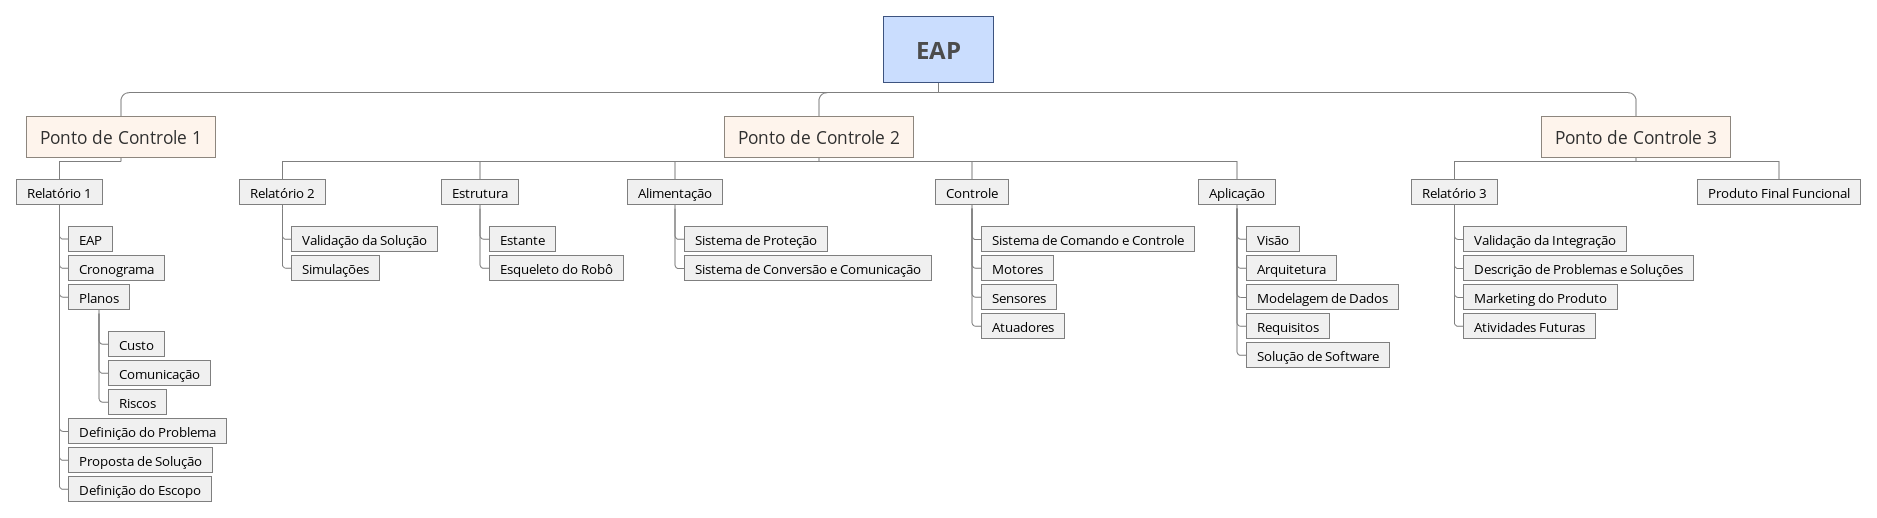
\includegraphics[scale=0.4, angle = 90]{figuras/eap}
\caption{Estrutura Analítica do Projeto}
\label{Estrutura Analítica do Projeto}
\end{figure}
\FloatBarrier


\section{Cronograma}
O Cronograma é o artefato responsável por registrar quais atividades deverão ser executadas em qual período de tempo. Através dele é possível perceber identificar atrasos no projeto.

Além disso no Cronograma também é designado o responsável pela atividade, que pode ser uma pessoa ou um grupo, caso haja a necessidade da visão colaborativa de outros membros



